\section{Setup}
\begin{figure}[ht]
\centering
\import{qcm/figures/}{qcm_annotated_picture.pdf_tex}
\caption{Annotated picture of the prototype CF-QCM, from above.  The
centrifuge is a standard swinging bucket type.}
\label{fig:cfqcmexpsetup}
\end{figure}

The CF-QCM experimental setup is shown in \Figure{fig:cfqcmexpsetup}.  It
consists of a \SI{25}{\milli\meter} diameter \SI{5}{\mega\hertz} gold
coated crystal in combination with an SRS QCM200 PLL based driver circuit
and an external rubidium frequency standard.  The driver circuit and
crystal are integrated into the arm of a commercial swinging bucket
centrifuge.  The QCM is then connected in proximity to a remote driver
which is tethered via a slip-ring connector to external data acquisition
electronics and a computer.  The crystal itself is mounted in a holder
radially by its edges such that the centrifugal force $F_\mathrm{c}$ is
always normal to the surface of the crystal.  On the sensing side of the
crystal is a $\SI{125}{\micro\liter}$ volume PDMS/glass cell containing the
sample.  The cell is made of a thin o-ring of PDMS (Sylgard 184, 10:1
ratio, cured \SI{20}{\minute} at \SI{120}{\celsius})
$\text{OD}=\SI{25}{\milli\meter}$, $\text{ID}=\SI{15.5}{\milli\meter}$ in
contact with the sensing side of the crystal and covered with
\SI{25}{\milli\meter} round N\raisebox{0.25em}{\relsize{-2}\b{o}}~1
coverglass, nominal thickness \SI{0.15}{\milli\meter}.  The non-sensing
side of the crystal remains in air and is isolated from the body of the
centrifuge.  

When in operation, the crystal and cell are mounted in either the
\textit{loading} configuration, where the centrifugal force is \textit{in
to} the sensing side or, by mounting it upside down, in the
\textit{unloading} configuration, where the force is \textit{away from} the
sensing side.

In addition to the standard QCM driver output, the computer simultaneously
records the angular velocity and internal temperature of the centrifuge
itself.  The angular velocity is obtained with an optical interrupter
switch placed over the spokes of an internal gear, acting as an ersatz
wheel encoder.  The temperature is obtained with a standard K-type
thermocouple.

The internal motor of the centrifuge was also interfaced to an external DC
power supply whose voltage was controlled by the same computer.  In this
way, the spin speed and acceleration could be controlled.

\begin{figure}[ht]
\centering
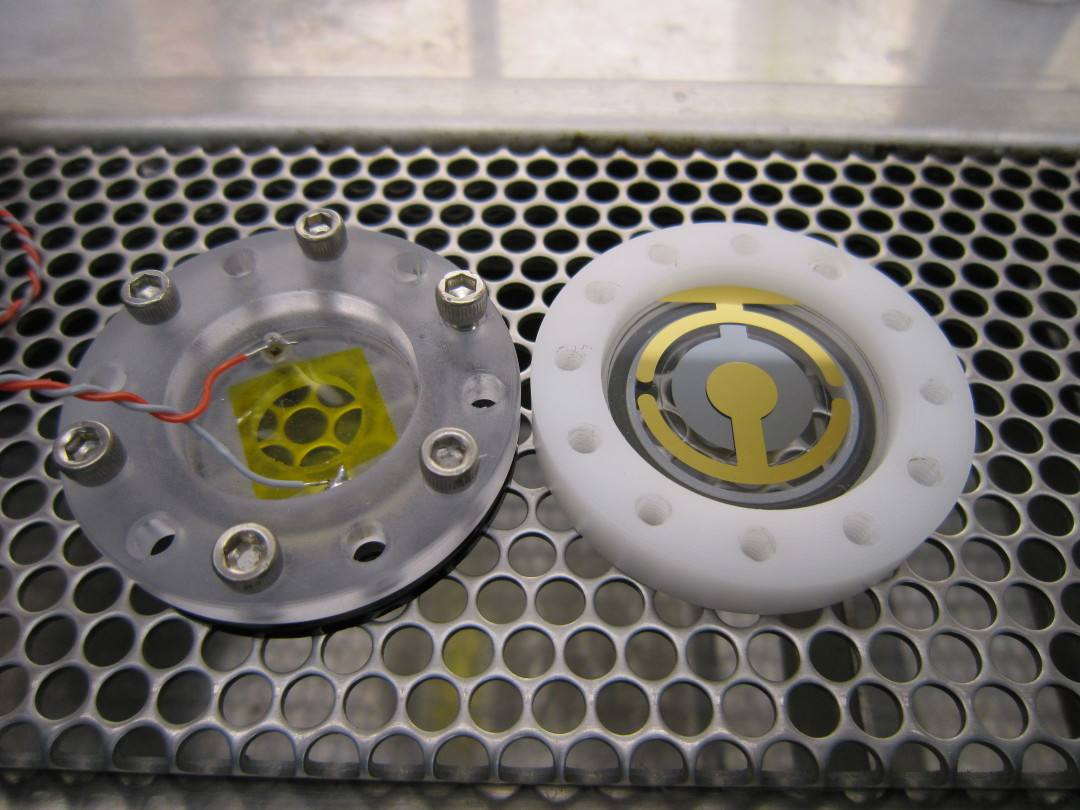
\includegraphics[width=10cm,keepaspectratio]{qcm/figures/qcm_holderdiss.jpg}
\caption{Holder for the crystal, shown here split into its two halves.  The
crystal is shown on the right.}
\label{fig:cfqcmexpsetup}
\end{figure}

\section{Noise and Comparison to QCM-D} \label{sec:suppqcmdcomp}
Typical of most QCM circuits, the QCM200 provides an output proportional to
$\df$, which we use directly in all discussions of $\df$.  However, unlike
a QCM-D device which gives a ``dissipation factor'', $D$, defined in
terms of the bandwidth $\dg$ as $D=2\dg/f_\mathrm{F}$, the QCM200
outputs the motional resistance $\Rm$ of the Butterworth van Dyke
equivalent circuit.  $\Rm$ is, related to
the bandwidth $\Gamma$ and the QCM-D dissipation $D$ by 
\begin{align}
 \Rm&=\left(4 \pi \Lm\right) \Gamma\\
 &=\left(2 \pi \Lm f_\mathrm{F}\right) D
\end{align}
where $\Lm$ is the Butterworth van Dyke equivalent motional inductance.
Because of the small load approximation, $\df/f_\mathrm{F} \ll 1$ and
likewise $\Delta L/\Lm \ll 1$, we can effectively treat $\Lm$ as a
constant.~\cite{geelhood2002transient}
This value is
typically in the range of
\SI{30}{\milli\henry}~\cite{srsqcm200manual}~\cite{hussain2005ots} to
\SI{40}{\milli\henry}~\cite{gottschling2000detection}~\cite{arnau2002circuit}~\cite{snellings2001response},
with \SI{40}{\milli\henry} being more common and the value we use in our
analysis.  At $\Lm=\SI{40}{\milli\henry}$, we find in water
$\Rm=\SI{359}{\ohm}$, which is within \SI{1}{\percent} of the predicted
value~\cite{kanazawa1985frequency} of \SI{357}{\ohm}.  In this sense,
dissipation $D$ and motional resistance $\Rm$ are independent but
equivalent measures of the QCM bandwidth.

We have calculated the noise in $\df$ and $\Rm$ for the SRS QCM200 in our
experiment and find it to be about \SI{0.4}{\hertz} (\SI{0.008}{ppm}) for
$\df$ and \SI{0.006}{\ohm} (\SI{13}{ppm}) for $\Rm$, corresponding to a
signal to noise ratio of \SI{110}{\decibel}.  This is close to the
manufacturer's specification~\cite{srsqcm200manual} of \SI{0.1}{\hertz} for
$\df$ and $\pm\SI{28}{ppm}$ for $\Rm$.  We have analyzed the noise
separately for both the loading and unloading orientations of the crystal,
as well as for different centrifuge spin speeds.  We find no discernible
difference in the noise between any of these cases.  We did not at any
point modify the centrifuge or bucket assembly in an attempt to try and
reduce system noise.

In comparison, a typical QCM-D such as those sold by
Q-Sense~\footnote{BiolinScientific / Q-Sense, Hängpilsgatan 7, SE-426 77
Västra Frölunda, Sweden,  \url{http://www.q-sense.com/}} will have noise of
about \SI{0.3}{\hertz} in $\df$ and \num{0.2e-6} in $D$ at
\SI{5}{\mega\hertz}~\cite{su2005comparison}~\cite{peh2007understanding}.
Converting from $\Rm$ to $D$ and vice-versa, we find the SRS QCM200 has an
equivalent noise in $D$ of \num{0.005e-6} and the Q-Sense QCM-D an
equivalent noise in motional resistance of \SI{0.25}{\ohm}.  In terms of
$\dg$, the Q-Sense QCM-D has a noise of \SI{0.5}{\hertz} and the SRS QCM200
\SI{0.01}{\hertz}.  Even though we stated that our chosen value for $\Lm$
gives $\Rm$ within \SI{1}{\percent} of the predicted value for water,
uncertainties in the value of $\Lm$ used for the $\Rm$-$\dg$ conversion do
not significantly affect this analysis for the range of $\Lm$ values quoted
in the literature.

It is clear with this comparison that the SRS QCM200 PLL based driver and a
QCM-D device are both measures of the same underlying physical phenomena
taking place in a resonating quartz crystal.~\cite{geelhood2002transient}
Moreover, as exemplified by the discrete particle data in the main text,
the QCM signal amplitudes increase further with the application of
centrifugal force for the device reported here.  It is important to note
that the important aspect of the CF-QCM, the centrifugal force, is
independent of the type of technique used to drive and monitor the quartz
crystal.  We therefore see no reason why our technique would not apply to
all QCM based measurement techniques.  

\section{Chemistry}
The quartz crystals are always cleaned before use by immersion
in fresh piranha solution (3:1 mixture of \SI{97}{\percent} \ce{H2SO4} and
\SI{30}{\percent} \ce{H2O2}) for \SI{5}{\minute} and rinsing liberally with
pure water.

Free particles (Spherotech SVP-10-5, SVM-15-10, and SVP-200-4), of
different diameters were prepared by diluting a solution of
\SI{30}{\micro\liter} particles in \SI{300}{\micro\liter} \ce{H2O}.  A
\SI{125}{\micro\liter} aliquot of the \SI{300}{\micro\liter} volume was
then placed in the PDMS cell in contact with the sensing side of the
crystal.  The sensing area was calculated to be
\SI{1.195}{\centi\meter\squared}.  The particles in solution experience a
buoyant force which reduces their apparent mass. The surface density
$N_\mathrm{L}$ was determined by counting the average number of particles
per unit area with a microscope and was found to be within
\SI{20}{\percent} of the value predicted by the volume concentration.

For experiments involving oligos, the crystals were first immersed in a
\SI{1}{\micro\textsc{M}} solution of thiolated oligos (5'-ThioMC6-TTT TTT
TTT CAC TAA AGT TCT TAC CCA TCG CCC-3') in a \SI{1}{\textsc{M}} potassium
phosphate buffer, \SI{0.5}{\textsc{M}} \ce{KH2PO4}, pH 3.8 for
\SI{1}{\hour}.  Following, immersion in \SI{1}{\milli\textsc{M}}
6-Mercapto-1-hexanol (MCH) was used to block residual reactive sites on the
gold electrode.  After rinsing, attachment to the prepared particles was
done in STE buffer: \SI{1}{\textsc{M}} \ce{NaCl} with
\SI{10}{\milli\textsc{M}} Tris buffer, pH 7.4 and \SI{1}{\milli\textsc{M}}
EDTA\@.  A complimentary strand (5'-biotin-CT CAC TAT AGG GCG ATG GGT AAG
AAC TTT AGT-3') was attached to the streptavidin coated particles.  The
particles were first washed two times by alliquoting a
\SI{100}{\micro\liter} base solution of particles in \SI{100}{\micro\liter}
STE buffer, \SI{5000}{RPM} for \SI{3}{\minute} and decanting the
supernatant.  The particles were resuspended in \SI{20}{\micro\liter} of
STE buffer and \SI{10}{\micro\gram} of oligos were added.  The mixture was
incubated \SI{15}{\minute} at room temperature under slow vortexing, then
washed again and resuspended in \SI{100}{\micro\liter} STE buffer.  The
oligo attached particle suspension was allowed to attach to the gold
surface for \SI{15}{\minute} before spinning.
 
Lambda DNAs were prepared by combining \SI{50}{\micro\liter} of lambda DNA
at \SI{500}{\micro\gram\per\milli\liter}, \SI{5.5}{\micro\liter} of 10x T4
ligase, and \SI{0.5}{\micro\liter} of diluted \SI{10}{\micro\textsc{M}}
thiolated linker oligonucleotide and heating to \SI{70}{\celsius} for
\SI{5}{\minute}.  The suspension was left to cool to room temperature as
the litigation of the oligos to the DNA COS ends occured. Once the mixture
was at room temperature, \SI{15}{\micro\liter} 10x ligase buffer,
\SI{127}{\micro\liter} \ce{H2O}, and \SI{2}{\micro\liter} T4 DNA ligase was
added to the annealed linker.  The reaction was allowed to proceed at room
temperature for \SI{3}{\hour}.

\section{Environmental Effects and Noise}
In the next chapter we will present the response of the CF-QCM under
different load situations.  Before doing so, it is prudent that all
non-sample phenomena that could influence the sensogram are taken into
account.  These have been tabulated in \Table{tbl:environmentaleffects}.
We will discuss this table in the next chapter.
\begin{table}
\centering
\begin{tabular}{l>{\raggedright}p{5cm}llllll}
\textbf{phenomena} & \textbf{response} & \textbf{refs} & \multicolumn{5}{l}{\textbf{predicted shifts}}\tabularnewline
 &  &  & \multicolumn{2}{l}{max} & \multicolumn{3}{l}{avg}\tabularnewline
 &  &  & $f$ & $R$ & $f$ & \multicolumn{2}{l}{$R$}\tabularnewline
temperature & \SI{8}{\hertz\per\celsius} and \SI{4}{\ohm\per\celsius} in water & \cite{srsqcm200manual} & 10.3768 & -5.1884 & 1.97248 & \multicolumn{2}{l}{-0.98624}\tabularnewline
 & Third order polynomial with maximum arount \SI{24}{\celsius} with
$a_1=\num{2.3888}$, $a_2=\num{-1.8719e+02}$, $a_3=\num{4.8587e+03}$,
$a_4=\num{-4.1814e+04}$. & \cite{reipa2006long} & 76.195 & - & 14.176 & \multicolumn{2}{l}{-}\tabularnewline
electric field & negligible  & \cite{walls1995fundamental} & $\sim0$ & $\sim0$ & $\sim0$ & \multicolumn{2}{l}{$\sim0$}\tabularnewline
magnetic field & \SI{10}{\per\tesla} for fields smaller than \SI{10}{\tesla} & \cite{walls1995fundamental} & $\sim0$ & $\sim0$ & $\sim0$ & \multicolumn{2}{l}{$\sim0$}\tabularnewline
pressure & \SI{-2970}{\hertz\centi\meter\squared\per\kilo\gram} for changes
to \SI{+2.1}{\kilo\gram\per\centi\meter\squared} & \cite{reipa2006long} & 30.02 & - & 20.01 & \multicolumn{2}{l}{-}\tabularnewline
 & \SI{-1458}{\hertz\centi\meter\squared\per\kilo\gram} (\SI{10}{\mega\hertz}
crystal) & \cite{heusler1988measurement} & 14.73 & - & 9.82 & \multicolumn{2}{l}{-}\tabularnewline
mechanical stress & $\Delta f = 1.62 g_f^{1.72}$ for two point symmetrical mounting in
air & \cite{fletcher1979comparison} & n/a & n/a & n/a & \multicolumn{2}{l}{n/a}\tabularnewline
sedimentation potential &  &  &  &  &  & \multicolumn{2}{l}{}\tabularnewline
parasitic capacitance & \SI{2}{\hertz\per\pico\farad} & \cite{srsqcm200manual} & ? & ? & ? & \multicolumn{2}{l}{?}\tabularnewline
 & \SI{0.825}{\hertz\per\pico\farad} (BvD analysis) & \cite{webster2013} & ? & ? & ? & \multicolumn{2}{l}{?}\tabularnewline
acceleration & \SI{9e-11}{\per g}, depending on orientation & \cite{norton1993tactical} & 0.9 & - & 0.045 & \multicolumn{2}{l}{-}\tabularnewline
 & \SI{0.0218813}{\hertz\per g} in air & \cite{1536938} & 4.3763 & - & 2.1881 &  & -\tabularnewline
\end{tabular}
\caption{Environmental effects on the QCM resonance frequency.}
\label{tbl:environmentaleffects}
\end{table}
